\lecture{Introdução}{intro}

\lecturetitle{\course}{\insertlecture}

\frame{\maketitle}

\section*{\insertlecture}



% \begin{frame}{O que é Engenharia de Software}
  
%   \begin{description}
%   \item[Engenharia:]
%     \href{http://www.thefreedictionary.com/engineering}{Aplicação dos
%       princípios {\bf matemáticos} e {\bf científicos} para fins práticos tais
%       como o projeto, manufatura e operação de estruturas, máquinas,
%       processos e sistemas {\bf eficientes} e {\bf econômicos}.}

%   \item[Software:]~conjunto de instruções para o computador para
%     executar tarefas e manipular dados.

%   \item[Engenharia de Software:]~Aplicação dos princípios {\bf
%       matemáticos} e {\bf científicos} para o projeto, implementação e
%     operação de conjunto de instruções para o computador.
%   \end{description}

% \end{frame}

% \begin{frame}{O que é Engenharia de Software}

%   \note{A definição apresentada não é totalmente aplicável à Engenharia de
%   Software, pois, alguns projetos aplicam métodos de produção
%   empíricos, ou seja, baseados na experiência.}
  
%   Uma definição mais
%   adequada é a formulada por Carvalho \& Chiossi~\cite{carvalho2001},
%   como sendo:

%   \begin{quote}
%     Uma disciplina que reúne metodologias, métodos e ferramentas a ser
%     utilizados, desde a percepção do problema até o momento em que o
%     sistema desenvolvido deixa de ser operacional, visando resolver
%     problemas inerentes ao processo de desenvolvimento e ao produto de
%     software.
%   \end{quote}
% \pause
%   Porém, o objetivo continua sendo o mesmo da Engenharia, tornar o
%   processo de produção de software eficiente e econômico.

% \end{frame}

\begin{frame}{Crise do Software}

  A ineficiência dos softwares e atrasos constantes de entrega,
  tornando-os financeiramente custosos, produziu o termo ``Crise do
  Software'', cunhado em 1968 durante a Conferência de Engenharia de
  Software da OTAN (Organização do Tratado do Atlântico Norte)
  realizada na Alemanha. Segundo Dijkstra, esta crise está relacionada
  ao aumento do poder de processamento das
  máquinas~\cite{humble:dijkstra1972}.

\end{frame}

%%% Matéria sobre a Apollo 11
% https://qz.com/726338/the-code-that-took-america-to-the-moon-was-just-published-to-github-and-its-like-a-1960s-time-capsule/

\begin{frame}{Software de controle de navegação: Apollo~11 (1969)}
  \footnotesize
  \begin{itemize}
  \item Tempo de desenvolvimento: 1961--1972.
  \item Coordenação: Margaret Hamilton, MIT.
  \item Linguagem: Assembly. O código fonte está disponível em  \url{https://github.com/chrislgarry/Apollo-11/}.
  \end{itemize}

  \begin{columns}
    \begin{column}{.5\textwidth}
     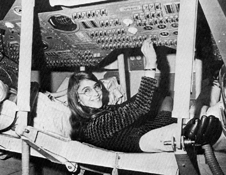
\includegraphics[scale=.6]{img/margaret-in-action.png}      

      \vfill
      {\tiny Fonte: \href{https://en.wikipedia.org/wiki/File:Margaret_Hamilton.gif}{NASA}}
  
  \end{column}
\only<2>{
    \begin{column}{.5\textwidth}
      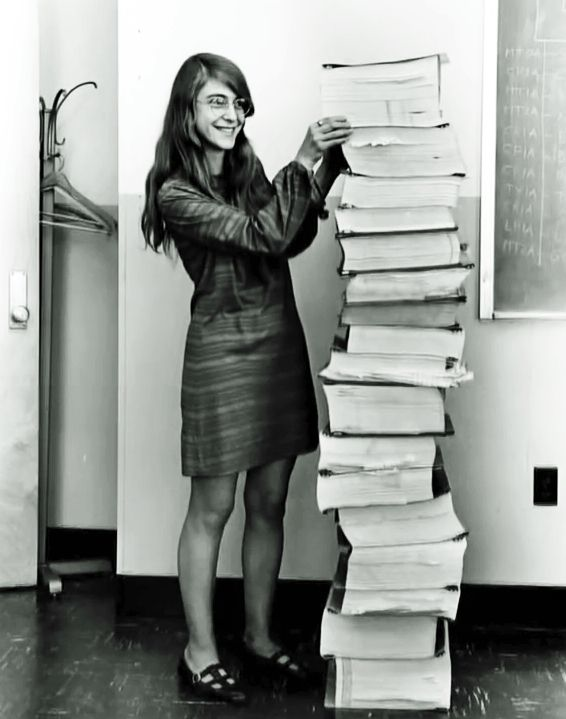
\includegraphics[scale=.22]{img/margaret.png}

      \vfill
      {\tiny Fonte: NASA via \href{https://en.wikipedia.org/wiki/File:Margaret_Hamilton.gif}{Wikipedia}}      
    \end{column}
}
  \end{columns}

\end{frame}

\begin{frame}{Referências}
  \begin{thebibliography}{1}

  \bibitem{brooks1975}
    Frederick~{P.}\ Brooks.
    \newblock {\em The Mythical Man-Month}.
    \newblock Addison-Wesley, 1975.
    
  \bibitem{humble:dijkstra1972}
    Edsger~W. Dijkstra.
    \newblock The humble programmer.
    \newblock {\em Communication of the ACM}, 15(10):859--866, 1972.

  \end{thebibliography}

\end{frame}

%% 
% Local variables:
% mode: latex
% mode:auto-fill
% TeX-file: main
% End:
%%
